\section{Paquetes}
\subsection{Introducci\'on}


El lenguaje R es un lenguaje que est\'a muy fundamentado en la comunidad, esta contribuye al desarrollo, mejora y extensi\'on de este lenguaje. La unidad fundamental a la hora de compartir 
nuestro trabajo con la comunidad es el paquete. Es por ello por lo cual se va a desarrollar un estudio sobre c\'omo crear un paquete en el lenguaje R y c\'omo distribuirlo de forma que est\'e disponible para toda la comunidad y contribuir al desarrollo de este lenguaje.

CRAN es el principal repositorio de paquetes estables de R, del cual se descargar\'an la mayor\'ia de los paquetes necesarios para un proyecto.

Para mas informaci\'on a cerca de los paquetes de R ver \cite{rcore} y \cite{book}, de donde se ha obtenido al mayor parte de la informaci\'on necesaria para este estudio.
\subsection{Estructura de paquetes en R}

Un paquete (\textbf{package}) es una colecci\'on de funciones, datos y c\'odigo R que se almacenan en una carpeta 
conforme a una estructura bien definida y f\'acilmente accesible para R \cite{librR}.

Estos paquetes sirven para incrementar la potencia de R mejorando su funcionalidad base, o a\~nadiendo 
nuevas.
Un paquete en R no est\'a compuesto s\'olo del c\'odigo en dicho lenguaje, sino que tambi\'en incorpora m\'as ficheros, 
los cuales se van a detallar a continuaci\'on.\cite{rParaTodos}

La informaci\'on b\'asica sobre un paquete se proporciona en el archivo \textbf{DESCRIPTION}, donde se puede ver qu\'e hace 
el paquete, qui\'en es el autor o autores, qui\'en realizar\'a el mantenimiento, a qu\'e versi\'on pertenece la documentaci\'on... entre otros datos.

En el fichero \textbf{NAMESPACE} se deber\'an especificar todos aquellos objetos que ser\'an importados o exportados del paquete.

En \textbf{LICENSE}, se incluir\'a una copia de la licencia para informar al usuario.

Para finalizar con los ficheros, se podr\'a encontrar en algunos casos uno llamado \textbf{NEWS}, en el cual estar\'an 
incluidos los cambios que se realizan de una versi\'on a otra.

La carpeta \textbf{R} es el n\'ucleo de la estructura, aqu\'i se encuentran todos los archivos \textbf{\textbf{.R}} con el c\'odigo de las funciones que incluya dicho paquete.
Es recomendable no aglutinar todo el c\'odigo en un mismo archivo, sino separar las funciones que tienen relaci\'on 
o que cumplen cierta funcionalidad en archivos separados, as\'i como dar un nombre descriptivo a los archivos.

La carpeta \textbf{man} contiene los ficheros de ayuda, es decir, estos paquetes compondr\'an el \enquote*{Manual de referencia} 
del paquete. Cada uno de estos ficheros, se debe corresponder a cada uno de los archivos que se encuentran 
en la carpeta R, pero en este caso, su nombre sera \textbf{nombre\_del\_archivo\textbf{.R}d}.

En la carpeta \textbf{data} se encontrar\'an todos los ficheros de datos que se deseen incorporar al paquete. La extensi\'on 
de estos ficheros ser\'an \textbf{\textbf{.R}Data} o \textbf{\textbf{.R}da}.
Por \'ultimo, en la carpeta \textbf{inst} estar\'an todos aquellos ficheros que se quiera que se instalen con el paquete.
\subsection{Requisitos previos}

\begin{itemize}
    \item R Studio
    \item Paquete \textbf{devtools}
    \item Paquete \textbf{\textbf{roxygen2}} 
    \item Rtools
\end{itemize}

\subsection{Crear proyecto R}

En este caso se puede hacer tanto con R Studio, como se muestra a continuaci\'on,
como con \textbf{devtools::create(}\enquote*{ruta/del/paquete/nombreDelPaquete}\textbf{)}, ambas opciones
proporcionar\'an un \enquote*{esqueleto} del paquete con los archivos imprescindibles.
Una vez abierto R Studio, lo primero que se debe hacer es crear un nuevo proyecto, para
ellos vamos a: 
\begin{center}
    \textbf{file > new project > new directory > r package} 
\end{center}

En la casilla \textbf{Package name:} se debe especificar el nombre del  proyecto; en la casilla
\textbf{Create package based on source files} se pueden a\~nadir (pinchar en el bot\'on \textbf{Add}) los
archivos \textbf{.R} que contengan nuestras funciones, si se han generado previamente (no es
estrictamente necesario a\~nadirlos ahora se pueden a\~nadir despu\'es).
Se ind\'ica el directorio ra\'iz en el que se situar\'a el subdirectorio en el que estar\'an
contenidos los archivos del proyecto. 
Al pinchar en el bot\'on \textbf{Create Project} se crear\'a un directorio en la ubicaci\'on indicada con la
estructura necesaria para que R pueda construir el paquete \cite{datavu}.

Una vez ajustada la configuraci\'on, hay que pinchar en \textbf{Install and Restart} de la pesta\~na \textbf{Build}, esto har\'a que \textbf{roxygen2} genere autom\'aticamente el archivo \textbf{.rd} de ayuda de nuestra funci\'on en la carpeta \textbf{man}.

\subsection{Documentaci\'on}
\textbf{[R Packages Hadley Wickman]}
La documentaci\'on es una de las partes m\'as importantes del paquete en R, ya que sirve para
ayudar a los usuarios a usar el paquete, para los desarrolladores que quieran extenderlo e
incluso para el propio creador del paquete, para en un futuro poder recordar para que serv\'ian
sus funciones.

Para qu\'e R pueda generar autom\'aticamente el archivo de ayuda para nuestras funciones
se va a hacer uso del paquete \textbf{roxygen2}, el cual se basa en la inclusi\'on de una serie de tags relacionados con el objetivo y descripci\'on de la funci\'on y/o paquete 


\begin{figure}[H]
    \centering
    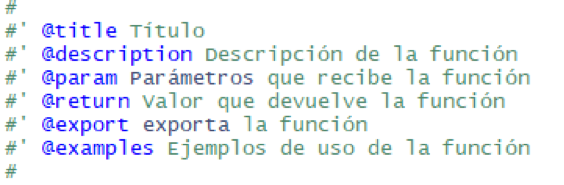
\includegraphics[scale=1]{Imagen_2}
    \caption{Ejemplo roxygen2   }
    \label{fig:roxygen}
\end{figure} 

Para ello se deben configurar las \textbf{Build Tools} de nuestro proyecto:

\begin{figure}[H]
    \centering
    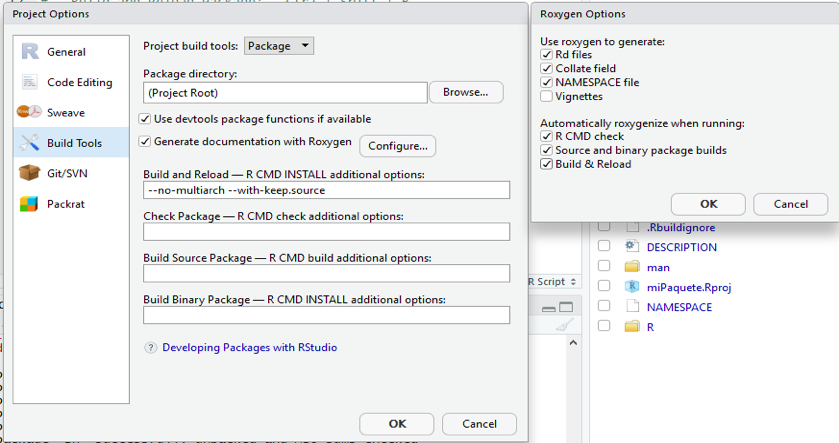
\includegraphics[scale=1]{Imagen_1}
    \caption{Configuraci\'on Build Tools }
    \label{fig:build_tools}
\end{figure} 

M\'as adelante se hablar\'a del uso del paquete \textbf{roxygen2} para generar la documentaci\'on del paquete

\subsubsection{Archivo DESCRIPTION}

En primer lugar, el archivo \textbf{DESCRIPTION} es lo que indica a R Studio que el directorio que lo
contiene es un paquete. Cuando se crea un proyecto e indicamos a R Studio que se va a
tratar de un paquete, este autom\'aticamente genera una plantilla del archivo \textbf{DESCRIPTION}
con los campos necesarios. De igual forma, si se crea el paquete haciendo uso de la herramienta \textbf{devtools}, se obtendr\'a
una plantilla similar.

\begin{figure}[H]
    \centering
    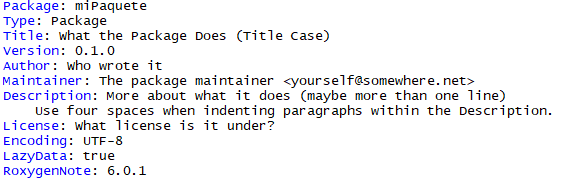
\includegraphics[scale=1]{pkge_metadata_1}
    \caption{Ejemplo Archivo DESCRIPTION }
    \label{fig:description}
\end{figure}

Este archivo usa un formato simple denominado \textit{Debian control format (DCF)} cuya estructura
es muy simple, cada l\'inea consiste en un campo y un valor separados por \enquote*{:}, cuando el valor
ocupa m\'as de una l\'inea hay que tabular las l\'ineas.

A parte de los campos de la plantilla existen otros m\'as a tener en cuenta como son \textbf{Imports}
y \textbf{Suggests}, ambos sirven para indicar las dependencias de nuestro paquete con respecto a otros.
Los principales campos de este archivo son: Package, Type, Title, Version, Author, Maintainer, Description y License.

La forma m\'as f\'acil de a\~nadir un paquete a \textbf{Imports} y \textbf{Suggests} es mediante el uso de
\textbf{devtools}, otra forma es haci\'endolo a mano en el archivo \textbf{DESCRIPTION}.

\begin{figure}[H]
    \centering
    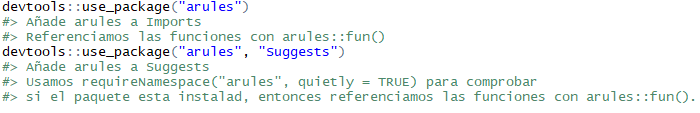
\includegraphics[scale=0.9]{pkge_metadata_6}
    \caption{Imports y Suggests con devtools }
    \label{fig:import_suggest}
\end{figure}

\subsubsection{Documentaci\'on de objetos}

En este caso se va a detallar la documentaci\'on de los distintos elementos que componen el
paquete.
Este tipo de documentaci\'on es accesible a trav\'es de \textbf{?} o \textbf{help()} y funciona como un
diccionario, permitiendo al usuario obtener informaci\'on sobre una funci\'on, paquete o conjunto
de datos.\\

\textbf{Crear la documentaci\'on}

Para crear esta documentaci\'on, lo primero que se debe hacer es a\~nadir comentarios
\textbf{roxygen} a los archivos \textbf{.R}, como, por ejemplo:

\begin{figure}[H]
    \centering
    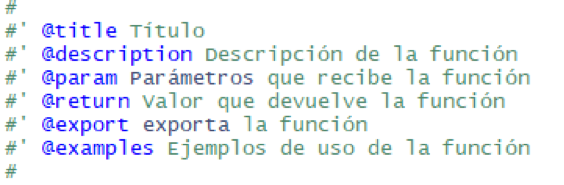
\includegraphics[scale=1]{Imagen_2}
    \caption{Ejemplo roxygen2   }
    \label{fig:roxygen2}
\end{figure} 

Una vez completado esto, presionamos \textbf{Ctrl/Cmd + Shift + B}, esto reconstruir\'a
completamente el paquete, actualizar\'a la documentaci\'on, reiniciar\'a R y recargar\'a \'el
paquete. \\

\textbf{Comentarios roxygen} \\
Estos comentarios comienzan con \textbf{\#'} y se colocan delante de cada funci\'on formando lo que
se llama un \textbf{bloque}. Estos bloques se dividen en \textbf{tags} (@NombreDelTag), el contenido de un
\textbf{tag} se extiende desde el final del nombre del tag hasta el inicio del siguiente o el final del
bloque.

Adem\'as, cada bloque incluye texto previo al primer tag, esto se denomina la introducci\'on y
se estructura de la siguiente forma:

\begin{itemize}
    \item La primera frase se corresponde con el t\'itulo de la documentaci\'on, es lo primero que
se ve cuando se consulta la ayuda de un paquete o funci\'on. Debe constar de solo
una l\'inea y acabar en punto.
    \item El segundo p\'arrafo es la descripci\'on, se muestra inmediatamente despu\'es del t\'itulo y
debe dar una breve descripci\'on de lo que hace la funci\'on.
    \item Por \'ultimo, el resto de p\'arrafos, si los hubiera, corresponden a una descripci\'on m\'as
detallada del funcionamiento de la funci\'on. Tambi\'en se puede usar el tag \textbf{@section}
para dividir los detalles de la funci\'on en distintas secciones.
\end{itemize}

El t\'itulo y la descripci\'on son obligatorios, mientras que los detalles son opcionales.
\textbf{Nota}: cada l\'inea de \textbf{roxygen} no debe superar los 80 caracteres y es recomendable tabular
las l\'ineas para facilitar la lectura.\\

\textbf{Documentando funciones} \\
Adem\'as del bloque introductorio y los tags ya mencionados, las funciones cuentan con una
serie de tags propios:
\begin{itemize}
    \item \textbf{@param} compuesto por un nombre y una descripci\'on. Sirve para describir los
par\'ametros de entrada de la funci\'on, su nombre, su tipo y para qu\'e se utilizan.
    \item \textbf{@examples} sirve para proveer c\'odigo en R que muestre un ejemplo de c\'omo funciona
la funci\'on. El c\'odigo debe funcionar sin errores. Esto es importante ya que muchos
usuarios miran primero los ejemplos.
    \item \textbf{@return} descripci\'on de la salida de la funci\'on.
\end{itemize}

\textbf{Documentando paquetes}\\
Se puede usar \textbf{roxygen} para crear una p\'agina de ayuda propia del paquete, no asociada a
una funci\'on en particular. Esta p\'agina es accesible mediante\\ \textbf{package?}\textit{nombreDelPaquete} y
puede ser usada para describir los componentes m\'as importantes del paquete o las
dependencias que tiene, por ejemplo.

En este caso, dado que no se corresponde con un objeto en concreto, se debe etiquetarlo
manualmente como \textbf{@docType package} y \textbf{@name} \textit{nombreDelPaquete} y poner un \textbf{NULL} al final.

\begin{figure}[H]
    \centering
    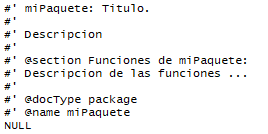
\includegraphics[scale=1]{od_1}
    \caption{Ejemplo documentaci\'on paquete }
    \label{fig:paquete}
\end{figure} 

\subsubsection{Datos externos}

Hay tres maneras principales de incluir datos en un paquete, dependiendo de qu\'e queramos
hacer con ellos o qui\'en debe usarlos:

\begin{itemize}
    \item Si se quiere almacenar datos binarios y que est\'en disponibles para los usuarios, se
deben poner en el directorio \textbf{data/}. Este es el mejor sitio para los datasets.
    \item Si lo que se quiere es almacenar datos de an\'alisis, pero que los dem\'as usuarios no
los tengan disponibles, se deben colocar en \textbf{R/sysdata.Rda}. En este caso es el mejor
sitio para los datos que necesiten nuestras funciones.
    \item Por \'ultimo, si queremos almacenar datos raw, se deben almacenar en el directorio
\textbf{inst/data}.
\end{itemize}

Si \textbf{DESCRIPTION} incluye LazyData: true, entonces los datasets se cargar\'an de forma
\enquote*{Lazy}. Es decir, que no ocupar\'an memoria hasta que se usen, \textbf{devtools::cr\'eate()} establece
\textbf{LazyData} a true autom\'aticamente.

\subsubsection{NAMESPACE}

El archivo \textbf{NAMESPACE} es muy importante en eñ paquete, ya que  ayuda a encapsular el paquete y que no falle por las dependencias que pueda tener de otros, ni
interfiera en otros que lo usen si lo actualizamos.

Como su nombre indica, \textbf{NAMESPACE} proporciona \enquote*{espacios para nombres}. Por ejemplo,
cuando se importan dos paquetes que ambos contienen una funci\'on con el mismo nombre,
se puede desambiguar con el operador \enquote*{::}. Por ejemplo, si se usan los paquetes \textit{plyr} ys
\textit{Hmisc}, ambos tienen la funci\'on \textbf{sumarize()}, por lo que, dependiendo de cu\'al se quiera usar,
se usar\'a \textbf{plyr::sumarize()} o \textbf{Hmisc::sumarize()}.

\textbf{NAMESPACE} hace el paquete autocontenido, tanto con los \textbf{Imports}, como con los
exports. Los \textbf{Imports}, definen c\'omo una funci\'on de un paquete encuentra una funci\'on de
otro. Los \textbf{exports}, ayudan a evitar los conflictos con otros paquetes especificando qu\'e
funciones se pueden usar fuera de nuestro paquete.\\

\textbf{El archivo NAMESPACE}

Cada l\'inea contiene una directriz: \textbf{S3method(), export(), exportClasses()}, adem\'as de otros.
Cada una de estas directivas describe un objeto de R, que nos indica si se exporta desde
el paquete para ser usado por los dem\'as o si se importa para usarlo de forma local.
En total hay ocho directrices. 

Cuatro de ellas describen las exportaciones:

\begin{itemize}
    \item \textbf{ export()}: exporta una funci\'on.
    \item \textbf{ exportPattern()}: exporta todas las funciones que coinciden con un patr\'on.
    \item \textbf{ exportClasses(), exportMethods()}: exporta las clases S4 y sus m\'etodos.
    \item \textbf{ S3method()}: exporta los m\'etodos de S3.
\end{itemize}

Y las cuatro restantes describen las importaciones:
\begin{itemize}
    \item \textbf{import()}: importa todas las funciones de un paquete.
    \item \textbf{importFrom()}: importa las funciones seleccionadas.
    \item \textbf{importClassesFrom(), importMethodsFrom()}: importa las clases S4 y sus
m\'etodos.
    \item \textbf{useDynLib()}: importa una funci\'on de C.
\end{itemize}

Generar el namespace con \textbf{roxygen2} es como generar la documentaci\'on para las funciones,
se usan los bloques y tags, a\~nadiendo los comentarios al \textbf{.R} correspondiente, se ejecuta
\textbf{devtools::document()} (o, \textbf{Ctrl + Shift +D}) y se comprueba que el archivo \textbf{NAMESPACE} se
haya modificado correctamente.\\

\begin{figure}[H]
    \centering
    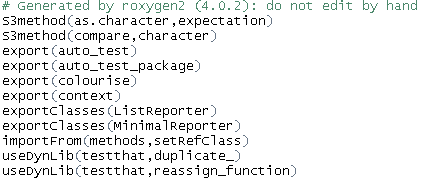
\includegraphics[scale=1]{namespace_2}
    \caption{Ejemplo de archivo NAMESPACE generado por roxygen2 }
    \label{fig:namespace}
\end{figure} 

\textbf{Exports}\\
Para que una funci\'on sea usable fuera de nuestro paquete debemos exportarla. Las funciones que se exporten deben estar documentadas.

\textbf{Imports}\\
\textbf{NAMESPACE} tambi\'en controla las funciones externas que pueden ser usadas en nuestro
paquete sin usar \enquote*{::}.

\subsection{Comprobando el paquete}

Una parte importante del desarrollo de un paquete es comprobar que el c\'odigo y la
documentaci\'on no presenten problemas, especialmente si se planea distribuir p\'ublicamente
el paquete. Para ello se tiene la herramienta que proporciona \textbf{devtools}, en concreto,
\textbf{devtools::check()} o, equivalentemente, \textbf{Ctrl + Shift + E} en R Studio.
Esta herramienta se encarga de que toda la documentaci\'on del paquete este actualizada, ya
que ejecuta \textbf{devtools::document()} de manera autom\'atica.

Encapsula el paquete antes de realizar las comprobaciones. Esto asegura que la
comprobaci\'on del paquete se hace desde un estado limpio ya que el encapsulamiento no
contiene ning\'un posible archivo temporal que se haya podido acumular y que pueda interferir
en las comprobaciones.\\

La mejor forma, aunque tediosa, de comprobar el paquete es la siguiente:

\begin{itemize}
    \item Ejecutar \textbf{devtools::check()} o \textbf{Ctrl + Shift + E} en R Studio.
    \item Arreglar el primer problema.
    \item Repetir los dos anteriores hasta que no haya m\'as problemas.
\end{itemize}

\textbf{devtools::check()} devuelve tres tipos de problemas distintos:

\begin{itemize}
    \item \textbf{Error}: Problema grave que deber ser arreglado, aunque no se planee subir el paquete a CRAN.
    \item \textbf{Warning}: Problema medio que debe ser arreglado en caso de que se planee subir el paquete a CRAN.
    \item \textbf{Note}: Problema medio que se deber\'ia arreglar en caso de querer subir el paquete a CRAN incluso si se trata de un falso positivo.
\end{itemize}


\subsection{Liberando el paquete}

Si se quiere que el paquete tenga cierta trascendencia en la comunidad de R, es necesario subirlo a CRAN, ya que la mayor\'ia de usuarios descargan e instalan sus paquetes desde CRAN.
A continuaci\'on, se detallar\'an las buenas pr\'acticas a la hora de distribuir el paquete a en CRAN. \\

\textbf{Comentarios CRAN}\\
Debemos recordar que CRAN est\'a compuesto por voluntarios que dedican parte de su tiempo
libre a revisar los paquetes que se suben, por tanto, cuanto m\'as f\'acil se les haga el trabajo,
m\'as posibilidades hay de que el paquete sea aceptado sin ning\'un problema.
Por ello, es recomendable a\~nadir al paquete una serie de comentarios que faciliten la tarea de revisi\'on, estos comentarios ir\'an en un archivo llamado \textbf{cran-comments.md}.

\begin{figure}[H]
    \centering
    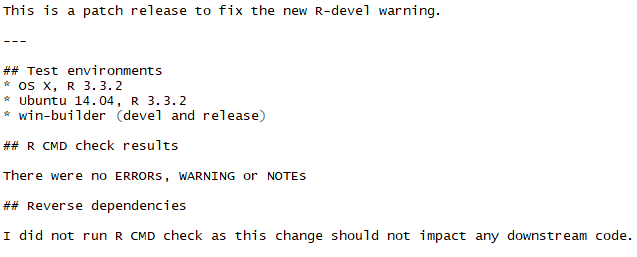
\includegraphics[scale=0.9]{rp_6}
    \caption{Comentarios CRAN}
    \label{fig:comentarios}
\end{figure} 
\begin{itemize}

    \item \textbf{Test environments}: indica en qu\'e plataformas se ha comprobado el paquete.
    \item \textbf{Check results}: contendr\'a una lista de errores, advertencias o notas.
    \item \textbf{Reverse dependencies}: sirve para indicar que si hay errores de dependencias con
otros paquetes en el caso de que se este  subiendo una nueva versi\'on del paquete y los cambios hayan provocado errores en las dependencias con otros paquetes.
\end{itemize}

\textbf{Las pol\'iticas en CRAN}\\
Existen ciertas pol\'iticas que debemos cumplir a la hora de subir el paquete a CRAN, estas son comprobadas manualmente. Algunos problemas comunes son:
\begin{itemize}
    \item Ausencia del email del mantenedor del paquete. 
    \item Es importante dejar claro los propietarios del copyright y si se ha usado c\'odigo externo, comprobar que la licencia es compatible.
    \item Paquetes que no funcionan en al menos dos plataformas no ser\'an considerados.
    \item No hacer cambios externos sin permiso del usuario: cambiar opciones, instalar paquetes, abrir software externo, cerrar R, etc.
    \item No subir actualizaciones del paquete muy frecuentemente. La pol\'itica sugiere hacerlo cada 1 o 2 meses como mucho.
\end{itemize}

\textbf{Archivos importantes}\\
Una vez que el paquete ya est\'a listo para subirlo, se deben  tener en cuenta dos archivos importantes m\'as,\textbf{ README.md}, el cual proporciona una descripci\'on del paquete y su
funcionamiento y uso, y \textbf{NEWS.md}, el cual describe los cambios con respecto a la versi\'on anterior del paquete. Dado que estos dos archivos no son soportados por CRAN no
hay que a\~nadirlos a la hora de construir el paquete
\begin{center}
    \textbf{devtools::use\_build\_ignore("NEWS.md")
    devtools::use\_build\_ignore("README.md")}
\end{center}


\textbf{Lanzamiento}

Lleg\'o la hora de construir el paquete y subirlo a CRAN. Para construir el paquete
usamos \textbf{devtools::release()}. Esto se encarga de volver a comprobar el paquete una \'ultima
vez y nos hace una serie de preguntas acerca de buenas pr\'acticas a modo de comprobaci\'on,
\textbf{devtools::release()}, autom\'aticamente, sube el paquete a CRAN.
Una vez subido, los voluntarios de CRAN comprobar\'an el paquete y
devolver\'an los resultados.
En caso de fallo, se deben resolver los problemas, y ejecutar \textbf{devtools::submit\_cran()} para evitar contestar de nuevo todas las preguntas de \\
\textbf{devtools::release()}.

\newpage